
\scnsuperset{системный sc-идентификатор}
\scnaddlevel{1}
\scnidtf{основной sc-идентификатор для языка общения между ostis-системами}
\scnaddlevel{1}
\scntext{примечание}{В качестве указанного языка общения между ostis-системами может использоваться SCs-код.}
\scnaddlevel{-1}
\scntext{примечание}{системный sc-идентификатор часто совпадает с основным англоязычным sc-идентификатором.}


\scnheader{sc-идентификатор}
\scnsubdividing{строковый sc-идентификатор\\
\scnaddlevel{1}
\scnidtf{sc-идентификатор, представленный строкой символов, которая является именем обозначаемой сущности}
\scnidtf{имя сущности, обозначаемой идентифицируемым sc-элементом}
\scnidtf{имя (термин, словосочетание), синонимичное соответствующему (идентифицируемому) sc-элементу и представленное в соответствующем алфавите символов}
\scnaddlevel{-1}
;sc-идентификатор, представленный иероглифами;sc-идентификатор, представленный условным обозначением или пиктограммой}
\scntext{примечание}{Введенные нами sc-идентификаторы используются во всех внешних языках, близких SC-коду -- в SCg-коде, в SCs-коде и в SCn-коде.}

\scnsegmentheader{Понятие простого идентификатора sc-элемента}

\scnstartsubstruct

\scnheader{простой идентификатор sc-элемента}
\scntext{правила построения}{Правила построения простых sc-идентификаторов.\\
Данные правила включают в себя:
\begin{scnitemize}
    \item Символы, используемые в простых sc-идентификаторах (в том числе, специальные символы);
    \item Специальные предикаты, используемые в простых sc-идентификаторах;
    \item Специальные суффиксы, используемые в простых sc-идентификаторах;
    \item Разделители, используемые в простых sc-идентификаторах;
    \item Ограничители, используемые в простых sc-идентификаторах;
    \item Правила построения простых sc-идентификаторов, определяемые различными классами идентифицируемых сущностей;
    \item Правила построения sc-имен собственных и sc-имен нарицательных.
\end{scnitemize}
Общим правилом построения простых sc-идентификаторов является стремление максимально возможным образом использовать сложившуюся терминологию. Но при этом следует подчеркнуть, что необходимость исключения омонимии в sc-идентификаторах требует строгого формального \uline{уточнения} семантической интерпретации каждого используемого термина. Особо подчеркнем то, что в ostis-системах процесс построения новых терминов (sc-идентификаторов) и процесс совершенствования существующей терминологии по отношению к процессу развития ostis-систем, баз знаний, представленных в SC-коде, с технической точки зрения абсолютно не зависят друг от друга. Кроме того, следует помнить, что \uline{далеко не все} sc-элементы, входящие в состав базы знаний ostis-системы, должны иметь соответствующие им sc-идентификаторы (быть идентифицированными). Очевидно, что идентифицированными (именованными) должны быть все используемые понятия, вводимые в соответствующих предметных областях и специфицируемые соответствующими онтологиями. Идентифицированными также должны быть обладающие особыми свойствами ключевые экземпляры (элементы) некоторых понятий, различные социально значимые объекты (персоны, населенные пункты, географические объекты, страны, организации, библиографические источники и многое другое).\\
Рассмотрим правила построений простых sc-идентификаторов, определеяемые различными классами идентифицируемых сущностей:
\begin{scnitemize}
    \item Первым символом каждого простого sc-идентификатора и каждого сложного sc-идентификатора, идентифицирующего sc-переменную (переменный sc-элемент), является подчеркнутый пробел;
    \item Последним символом простого sc-идентификатора, идентифицирующего sc-узел, обозначающий неролевое отношение, заданное на множестве sc-элементов, является крестик в виде верхнего индекса;
    \item Последним символом простого sc-идентификатора, идентифицирующего sc-узел, обозначающий заданное на множестве sc-элементов ролевое отношение (т.е. отношение, являющееся подмножеством отношения принадлежности), является апостроф (черточка в виде верхнего индекса);
    \item Последним символом простого sc-идентификатора, идентифицирующего sc-узел, обозначающий понятие, не являющееся отношением, (таковыми, в частности, являются различного рода параметры — длина, площадь, объем, масса) является звездочка в виде верхнего индекса;
    \item В рамках SCs-кода целесообразно вводить правила унифицированного построения простых sc-идентификаторов и целого ряда других классов идентифицируемых сущностей — персон, библиографических источников (публикаций), разделов баз знаний ostis-систем, файлов ostis-систем, самих ostis-систем.
\end{scnitemize}}

\scnheader{имя нарицательное}
\scnidtf{имя, которое может быть приписано \uline{любому} экземпляру некоторого класса и которое обозначает указанный класс}
\scntext{примеры}{треугольник; город; персона; отношение; параметр; константа; переменная}
\scnnote{\textit{имя нарицательное} всегда начинается с маленькой буквы}

\scnheader{имя собственное}
\scnidtf{имя, которое либо не является обозначением какого-либо класса сущностей, либо является обозначением (именем) некоторого класса сущностей, но построенным без использования нарицательного имени этого класса, либо является именем некоторого класса сущностей, построенным с использованием нарицательного имени этого класса (1) путем преобразования имени нарицательного во множественное число или (2) путем дополнительного использования в начале формируемого имени собственнного таких терминов, как "Класс...", "Множество...", "Множество всевозможных...".}
\scntext{примеры}{Москва; Иванов Иван Сергеевич; Точка А; Город Минск; SC-код; Русский язык; Множество всевозможных sc-текстов; Класс sc-текстов; Класс русскоязычных текстов.}
\scnnote{имя собственное всегда начинается с большой буквы}

\scnendstruct

\scnsegmentheader{Понятие сложного идентификатора sc-элемента}

\scnstartsubstruct

\scnheader{сложный sc-идентификатор}
\scnsuperset{сложный sc-идентификатор, идентифицирующее sc-коннектор}
\scnsuperset{сложный sc-идентификатор, ограничиваемое фигурными скобками и обозначающее множество sc-элементов, все sc-идентификаторы которых перечисляются}
\scnsuperset{сложный sc-идентификатор, ограничиваемое фигурными скобками и обозначающее множество sc-элементов, входящих в состав sc-текста, который семантически эквивалентен тому тексту (sc.s-тексту, sc.g-тексту, ея-тексту и т.д.), который ограничен указанными фигурными скобками}
\scnsuperset{сложный sc-идентификатор, ограничиваемое квадратными скобками и обозначающее файл-экземпляр ostis-системы}
    \scnaddlevel{1}
    \scnrelfrom{смотрите}{Принципы SC-кода}
        \scnaddlevel{1}
        \scniselement{секция раздела базы знаний}
        \scnaddlevel{-1}
    \scnaddlevel{-1}
\scnsuperset{сложный sc-идентификатор, ограничиваемое квадратными скобками и дополнительными вертикальными линиями (или кавычками) и обозначающее файл-класс ostis-системы}
    \scnaddlevel{1}
    \scnrelfrom{смотрите}{Принципы SC-кода}
        \scnaddlevel{1}
        \scniselement{секция раздела базы знаний}
        \scnaddlevel{-1}
    \scnaddlevel{-1}
\scnsuperset{сложный sc-идентификатор, использующее знаки алгебраических операций}
    \scnaddlevel{1}
    \scntext{примеры}{($s_i \cup s_j \cup s_k$); ($s_i \cap s_j \cap s_k$); ($s_i \backslash s_j$); ($x+y+z$); ($x \times y \times z$)}
    \scnaddlevel{-1}
\scnsuperset{сложный sc-идентификатор, обозначающее второй компонент пары указываемого ориентированного бинарного или квазибинарного отношения для указываемых аргументов\\
    \scnaddlevel{1}
    \scntext{примеры}{объединение*($s_i$; $s_j$; $s_k$); пересечение*($s_i$; $s_j$; $s_k$); разность множеств*($s_i$; $s_j$); сложение*($x$; $y$; $z$); умножение*($x$; $y$; $z$); sin*($x$); cos*($x$)}
    \scnaddlevel{-1}}
\scnexplanation{Использование сложныйх sc-идентификаторов позволяет существенно сократить число "придумываемых"\ sc-идентификаторов, каковыми в конечном счете становятся только простые sc-идентификаторы, поскольку, зная то, как связан идентифицируемый sc-элемент с теми sc-элементами, которые уже имеют sc-идентификаторы, во многих случаях можно построить сложный sc-идентификатор, идентифицирующее указанный sc-элемент. Кроме того, каждое сложный sc-идентификатор, являясь внешним идентификатором, является также и \uline{транслируемым} формальным текстом, содержащим некоторую информацию об обозначаемой ею сущности.}

\scnheader{сложный sc-идентификатор, идентифицирующий sc-коннектор}
\scnnote{Поскольку кратные sc-коннекторы одного и того же вида встречаются редко, сложный sc-идентификатор, идентифицирующий sc-коннектор, чаще всего \uline{однозначно} идентифицирует соответствующий sc-коннектор. В случае кратных sc-коннекторов одинакового семантического вида, отражаемого типом sc.s-коннектора, можно, например, sc-идентификаторам, идентифицирующим разные кратные sc-коннекторы, приписывать разные номера. Пусть, например, sc-элементы $e_i$ и $e_j$ соединены двумя \uline{кратными} константными постоянными sc-дугами. Тогда указанные sc-дуги можно идентифицировать следующими sc-идентификаторами:\\
($e_i => e_j$)1\\
($e_i => e_i$)2\\}

\scnheader{Файл-рисунок на странице 125}
\scnexplanation{В данном файле ostis-системы приведено определение понятия сложный sc-идентификатор, идентифицирующий sc-коннектор, представленное в SCg-коде и на Языке Бэкуса-Наура.}

\scnheader{Таблица.Типология сложных sc-идентифкаторов}
\scneqfile{\\
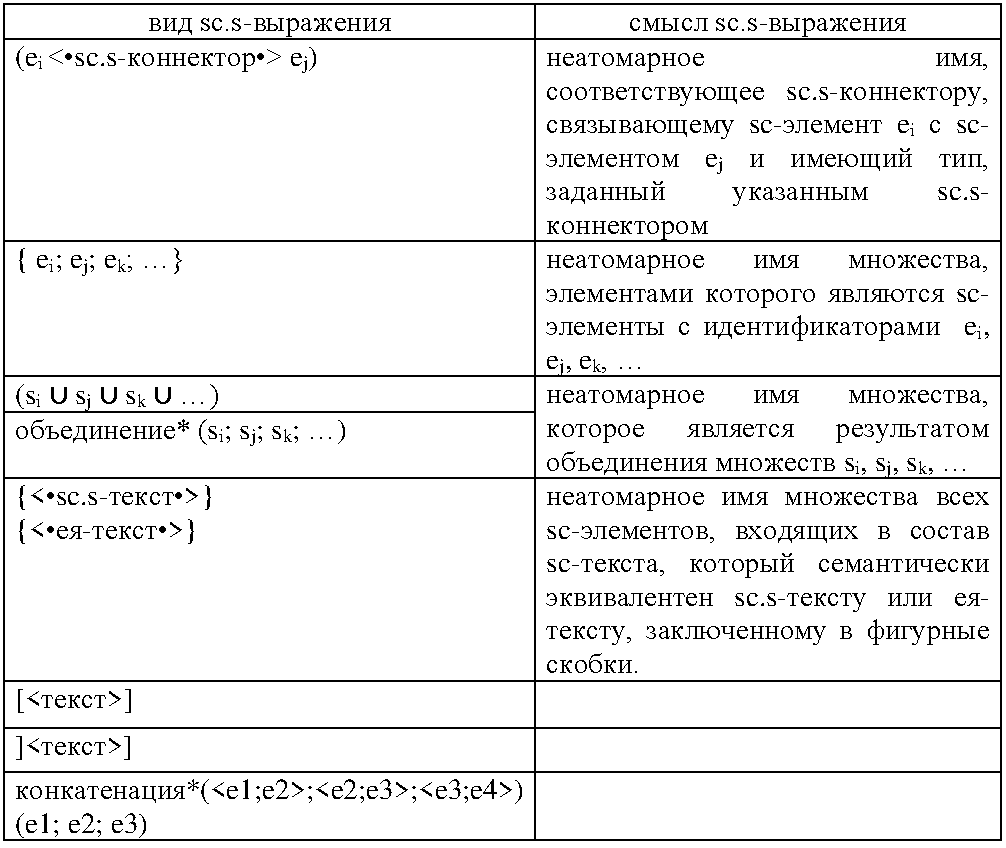
\includegraphics[width=1\linewidth]{figures/intro/scs-statements.pdf}\\
}

\scnendstruct \scninlinesourcecommentpar{Завершили представление Сегмента "\textit{Понятие сложного идентификатора sc-элемента}"}